\begin{pastexam}[label={px:ntu-110-comm-dsa-42}]{臺大電信所 110 學年度（B）第 42 題}
（複選；每題 2.5 分，每答錯一個選項倒扣 0.5 分至該題 0 分止）

Consider the splay tree in Figure 1. Which of the following statements are true?\\
(Assume bottom-up splay, also assume the Join() operation splays on the maximum element in the left tree, which then attaches the right tree.)
\begin{enumerate}[label=\Alph*.]
\item In Figure 1, after deleting key 26, then key 33 is a child of key 48.
\item In Figure 1, after deleting key 26, then key 17 is the root.
\item In Figure 1, after inserting key 75, then key 64 is an ancestor of key 99.
\item In Figure 1, after inserting key 75, then key 33 is a descendant of key 55.
\item In Figure 1, after inserting key 75, then key 75 is the root.
\end{enumerate}
\begin{center}
\begin{tikzpicture}[v/.style={circle,draw,thick,inner sep=1pt,minimum size=6mm,font=\small\sffamily},>={Stealth[length=2mm]}]
\node[v] (55) at (0,0) {55};
\node[v] (48) at (-0.9,-0.95) {48}; \node[v] (64) at (0.8,-0.95) {64};
\node[v] (33) at (-1.8,-1.9) {33}; \node[v] (82) at (1.7,-1.9) {82};
\node[v] (26) at (-2.7,-2.85) {26}; \node[v] (71) at (1.1,-2.85) {71}; \node[v] (99) at (2.3,-2.85) {99};
\node[v] (17) at (-3.45,-3.8) {17};
\foreach \a/\b in {55/48,55/64,48/33,33/26,26/17,64/82,82/71,82/99} \draw[thick,->] (\a) -- (\b);
\end{tikzpicture}
\\*[4pt] Figure 1: Splay tree
\end{center}
\end{pastexam}

\begin{pastsoln}
答案是 B、D、E。

由下而上的伸展（splay）把節點 $x$ 一路轉到根，每一步看 $x$、父節點 $p$、祖父節點 $g$（資結書第~10.6.1~節）：
\begin{itemize}
\item zig：$p$ 是根，對 $p$ 旋轉一次。
\item zig-zig：$x$、$p$ 同在左邊（或同在右邊），先轉 $g$、再轉 $p$。
\item zig-zag：一左一右，對 $p$ 轉、再對 $g$ 轉（和 AVL 的雙旋轉相同）。
\end{itemize}

\textbf{刪除 26}。 先把 $26$ 伸展到根，再拿掉它，剩下左樹 $L$ 和右樹 $R$，用 Join 接起來（資結書第~10.6.2~節）。
\begin{enumerate}
\item $26$ 是 $33$ 的左子、$33$ 是 $48$ 的左子：zig-zig。 先對 $48$ 右旋（$33$ 上來，$48$ 變成 $33$ 的右子），
再對 $33$ 右旋（$26$ 上來，$33$ 變成 $26$ 的右子）。 這一段變成 $26$（左 $17$，右 $33$，$33$ 的右是 $48$），
掛在 $55$ 的左邊。
\item $26$ 的父節點 $55$ 是根：zig，對 $55$ 右旋。 $26$ 成為根，$55$ 是它的右子，$26$ 原來的右子樹（$33$ 那段）
變成 $55$ 的左子樹。
\end{enumerate}
拿掉根 $26$：$L$ 只有 $17$，$R$ 是以 $55$ 為根、左邊 $33 \to 48$、右邊 $64 \to 82(71, 99)$ 的樹。 Join 把 $L$ 的
最大值 $17$ 伸展到 $L$ 的根（它本來就是），再把 $R$ 接成 $17$ 的右子樹：
\begin{center}
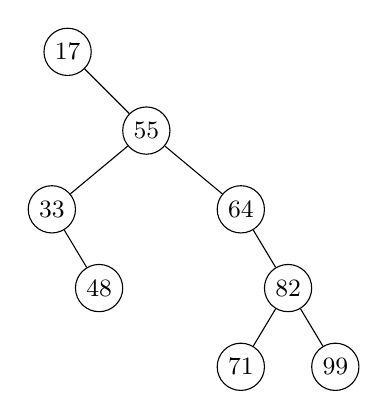
\begin{tikzpicture}[every node/.style={circle,draw,inner sep=1pt,minimum size=6mm,font=\small},level distance=10mm,edge from parent/.style={draw},level 1/.style={sibling distance=20mm},level 2/.style={sibling distance=24mm},level 3/.style={sibling distance=12mm}]
\node {17}
  child[missing]
  child {node {55}
    child {node {33} child[missing] child {node {48}}}
    child {node {64} child[missing] child {node {82} child {node {71}} child {node {99}}}}};
\end{tikzpicture}
\end{center}
\begin{itemize}
\item A 錯：$48$ 是 $33$ 的子節點，不是反過來。
\item B 對：根是 $17$。
\end{itemize}

\textbf{插入 75}。 先照二元搜尋樹插入：$75 > 55$、$> 64$、$< 82$、$> 71$，放在 $71$ 的右子。 再把 $75$ 伸展到根：
\begin{enumerate}
\item $75$ 是 $71$ 的右子、$71$ 是 $82$ 的左子：zig-zag。 $75$ 上來，左子 $71$、右子 $82$（$82$ 的右子仍是 $99$）。
\item 這時 $75$ 是 $64$ 的右子、$64$ 是 $55$ 的右子：zig-zig。 先對 $55$ 左旋（$64$ 成為根，$55$ 是它的左子），
再對 $64$ 左旋（$75$ 成為根，$64$ 是它的左子，$75$ 原來的左子 $71$ 變成 $64$ 的右子）。
\end{enumerate}
\begin{center}
\begin{tikzpicture}[every node/.style={circle,draw,inner sep=1pt,minimum size=6mm,font=\small},level distance=10mm,edge from parent/.style={draw},level 1/.style={sibling distance=36mm},level 2/.style={sibling distance=16mm},level 3/.style={sibling distance=12mm},level 4/.style={sibling distance=10mm}]
\node {75}
  child {node {64}
    child {node {55} child {node {48} child {node {33} child {node {26} child {node {17}} child[missing]} child[missing]} child[missing]} child[missing]}
    child {node {71}}}
  child {node {82} child[missing] child {node {99}}};
\end{tikzpicture}
\end{center}
\begin{itemize}
\item C 錯：$99$ 在 $82$ 底下，$82$ 是根 $75$ 的右子；$64$ 在左邊，不是 $99$ 的祖先。
\item D 對：$33$ 在 $55 \to 48 \to 33$ 這條路上，是 $55$ 的子孫。
\item E 對：伸展後新插入的 $75$ 就是根。
\end{itemize}
\end{pastsoln}
